\documentclass[conference]{IEEEtran}

\usepackage[T1]{fontenc}
\usepackage[utf8]{inputenc}
\usepackage{cite}
\usepackage{amsmath,amssymb,amsfonts}
\usepackage{graphicx}
\usepackage{booktabs}
\usepackage{array}
\usepackage{multirow}
\usepackage{url}
\usepackage{xcolor}
\usepackage{microtype}

\graphicspath{{figures/}}

\title{RoadMC: Physics-Guided Synthetic Point Clouds for Pavement Defect Segmentation}

\author{\IEEEauthorblockN{YQGHL}
\IEEEauthorblockA{RoadMC repository snapshot\\
\texttt{https://github.com/YQGHL/roadmc}}}

\begin{document}
\maketitle

\begin{abstract}
Road pavement defect segmentation in point clouds is limited by sparse annotations, severe class imbalance, and weak coverage of rare damage patterns. This report presents RoadMC, a physics-guided pipeline that synthesizes labeled pavement point clouds from road roughness spectra, micro-texture, explicit disease primitives, and a LiDAR observation model. The resulting scenes are consumed by a modular segmentation framework that supports either a Swin3D or PointMamba backbone, mHC hyper-connections, and a hybrid Muon/AdamW optimization strategy. On the held-out synthetic binary benchmark, the best calibrated checkpoint reaches 0.7319 mIoU, 0.7052 disease IoU, 0.9039 precision, and 0.7624 recall after threshold sweep. Pilot 38-class experiments remain unstable, motivating a staged training strategy that first stabilizes binary disease segmentation and then transfers to fine-grained categories.
\end{abstract}

\begin{IEEEkeywords}
point cloud synthesis, pavement defect segmentation, synthetic data, Swin3D, PointMamba, mHC, road damage
\end{IEEEkeywords}

\section{Introduction}
Road surface inspection is a classic yet still difficult perception problem. Fine-grained road defects such as cracks, potholes, rutting, and spalling are geometrically thin, long-tailed, and often expensive to annotate in large numbers. For this reason, synthetic point clouds are attractive: they can provide controlled geometry, balanced supervision, and scene-level repeatability.

This work is built around a simple premise: the synthetic generator is not a preprocessing script but a first-class part of the method. RoadMC uses a physics-guided synthesis stage to create labeled scenes, and a separate segmentation stage to validate whether the generated data actually supports learning. The current experimental path is binary first, then 38-class fine-tuning.

Our main contributions are:
\begin{itemize}
  \item a physics-guided pavement point-cloud synthesis pipeline that combines roughness spectra, micro-texture, defect primitives, and LiDAR-style observation;
  \item a modular segmentation stack with Swin3D or PointMamba backbones, optional mHC, and hybrid Muon/AdamW optimization;
  \item a pilot study showing that calibrated binary inference can reach 0.7319 mIoU on the held-out synthetic validation split.
\end{itemize}

\section{Related Work}
Point cloud learning has progressed from early hierarchical set abstraction to transformer and state-space backbones. PointNet++ introduced multi-scale local feature learning for unordered point sets \cite{pointnetpp}. Swin3D brought the Swin Transformer idea into 3D point cloud analysis with sparse voxel attention \cite{swin3d}. PointMamba transferred state-space modeling to point cloud analysis with linear complexity and a Morton-like ordering strategy \cite{pointmamba}. For imbalance-heavy detection and segmentation settings, focal-style reweighting remains a standard and effective choice \cite{focal}.

The mHC module adopted in RoadMC follows the recent hyper-connection line of work that restores a more stable identity mapping while still widening residual communication \cite{mhc}. In this report, mHC is used as an optional connector inside the segmentation backbone rather than as a standalone architecture.

\section{RoadMC Method}
\subsection{Point-Cloud Synthesis}
Given a road roughness field, RoadMC constructs a labeled point-cloud scene by composing the following elements:
\begin{equation}
S = \mathcal{G}(R, T, D, \mathcal{L}),
\end{equation}
where $R$ denotes the road surface roughness prior, $T$ denotes micro-texture, $D$ denotes defect primitives, and $\mathcal{L}$ denotes the LiDAR observation model.

The implementation follows six conceptual steps. First, the road base is drawn from an ISO 8608 power-spectral-density model so that the macro surface inherits realistic roughness statistics. Second, micro-texture is added by fractal perturbation and local curvature modulation. Third, defect primitives deform the surface to create cracks, potholes, rutting, spalling, and joint damage. Fourth, a scan-line LiDAR approximation transforms the surface into irregular sampled points. Fifth, point-wise labels are propagated from the defect regions into a JTG-style taxonomy. Sixth, scenes are exported as compressed ``.npz'' files containing points, labels, feats, normals, and pavement type.

\subsection{Segmentation Backbone}
The training stack shares a common input interface: normalized XYZ coordinates and three geometric features, namely intensity, curvature, and crack-boundary distance. The backbone can be configured as either:
\begin{itemize}
  \item \textbf{Swin3D}: a hierarchical window-attention network that operates on 3D point tokens and aggregates multi-scale skip features;
  \item \textbf{PointMamba}: a Morton-ordered scan mixer that replaces attention with sequence-style state updates.
\end{itemize}

Both backbones feed a shared decoder head. mHC can be enabled or disabled in the backbone blocks, making it easy to test whether residual channel mixing helps a specific backbone.

\subsection{Losses and Calibration}
Training uses a composite objective:
\begin{equation}
\mathcal{L} = \lambda_f \mathcal{L}_{\mathrm{focal}} + \lambda_d \mathcal{L}_{\mathrm{dice}} + \lambda_e \mathcal{L}_{\mathrm{edge}}.
\end{equation}
Focal loss addresses background dominance \cite{focal}, Dice loss stabilizes small-object learning, and a soft edge loss encourages boundary sensitivity around crack-like structures.

For binary inference, the positive-class probability is thresholded as
\begin{equation}
\hat{y}_i = \mathbb{1}\left[\mathrm{softmax}(z_i)_1 > \tau\right],
\end{equation}
where $\tau$ is selected by validation sweep. The best calibrated checkpoint in our experiments uses a threshold near $0.44$. Macro mIoU is reported with background excluded, matching the validation protocol used in the project logs.

\begin{figure*}[t]
  \centering
  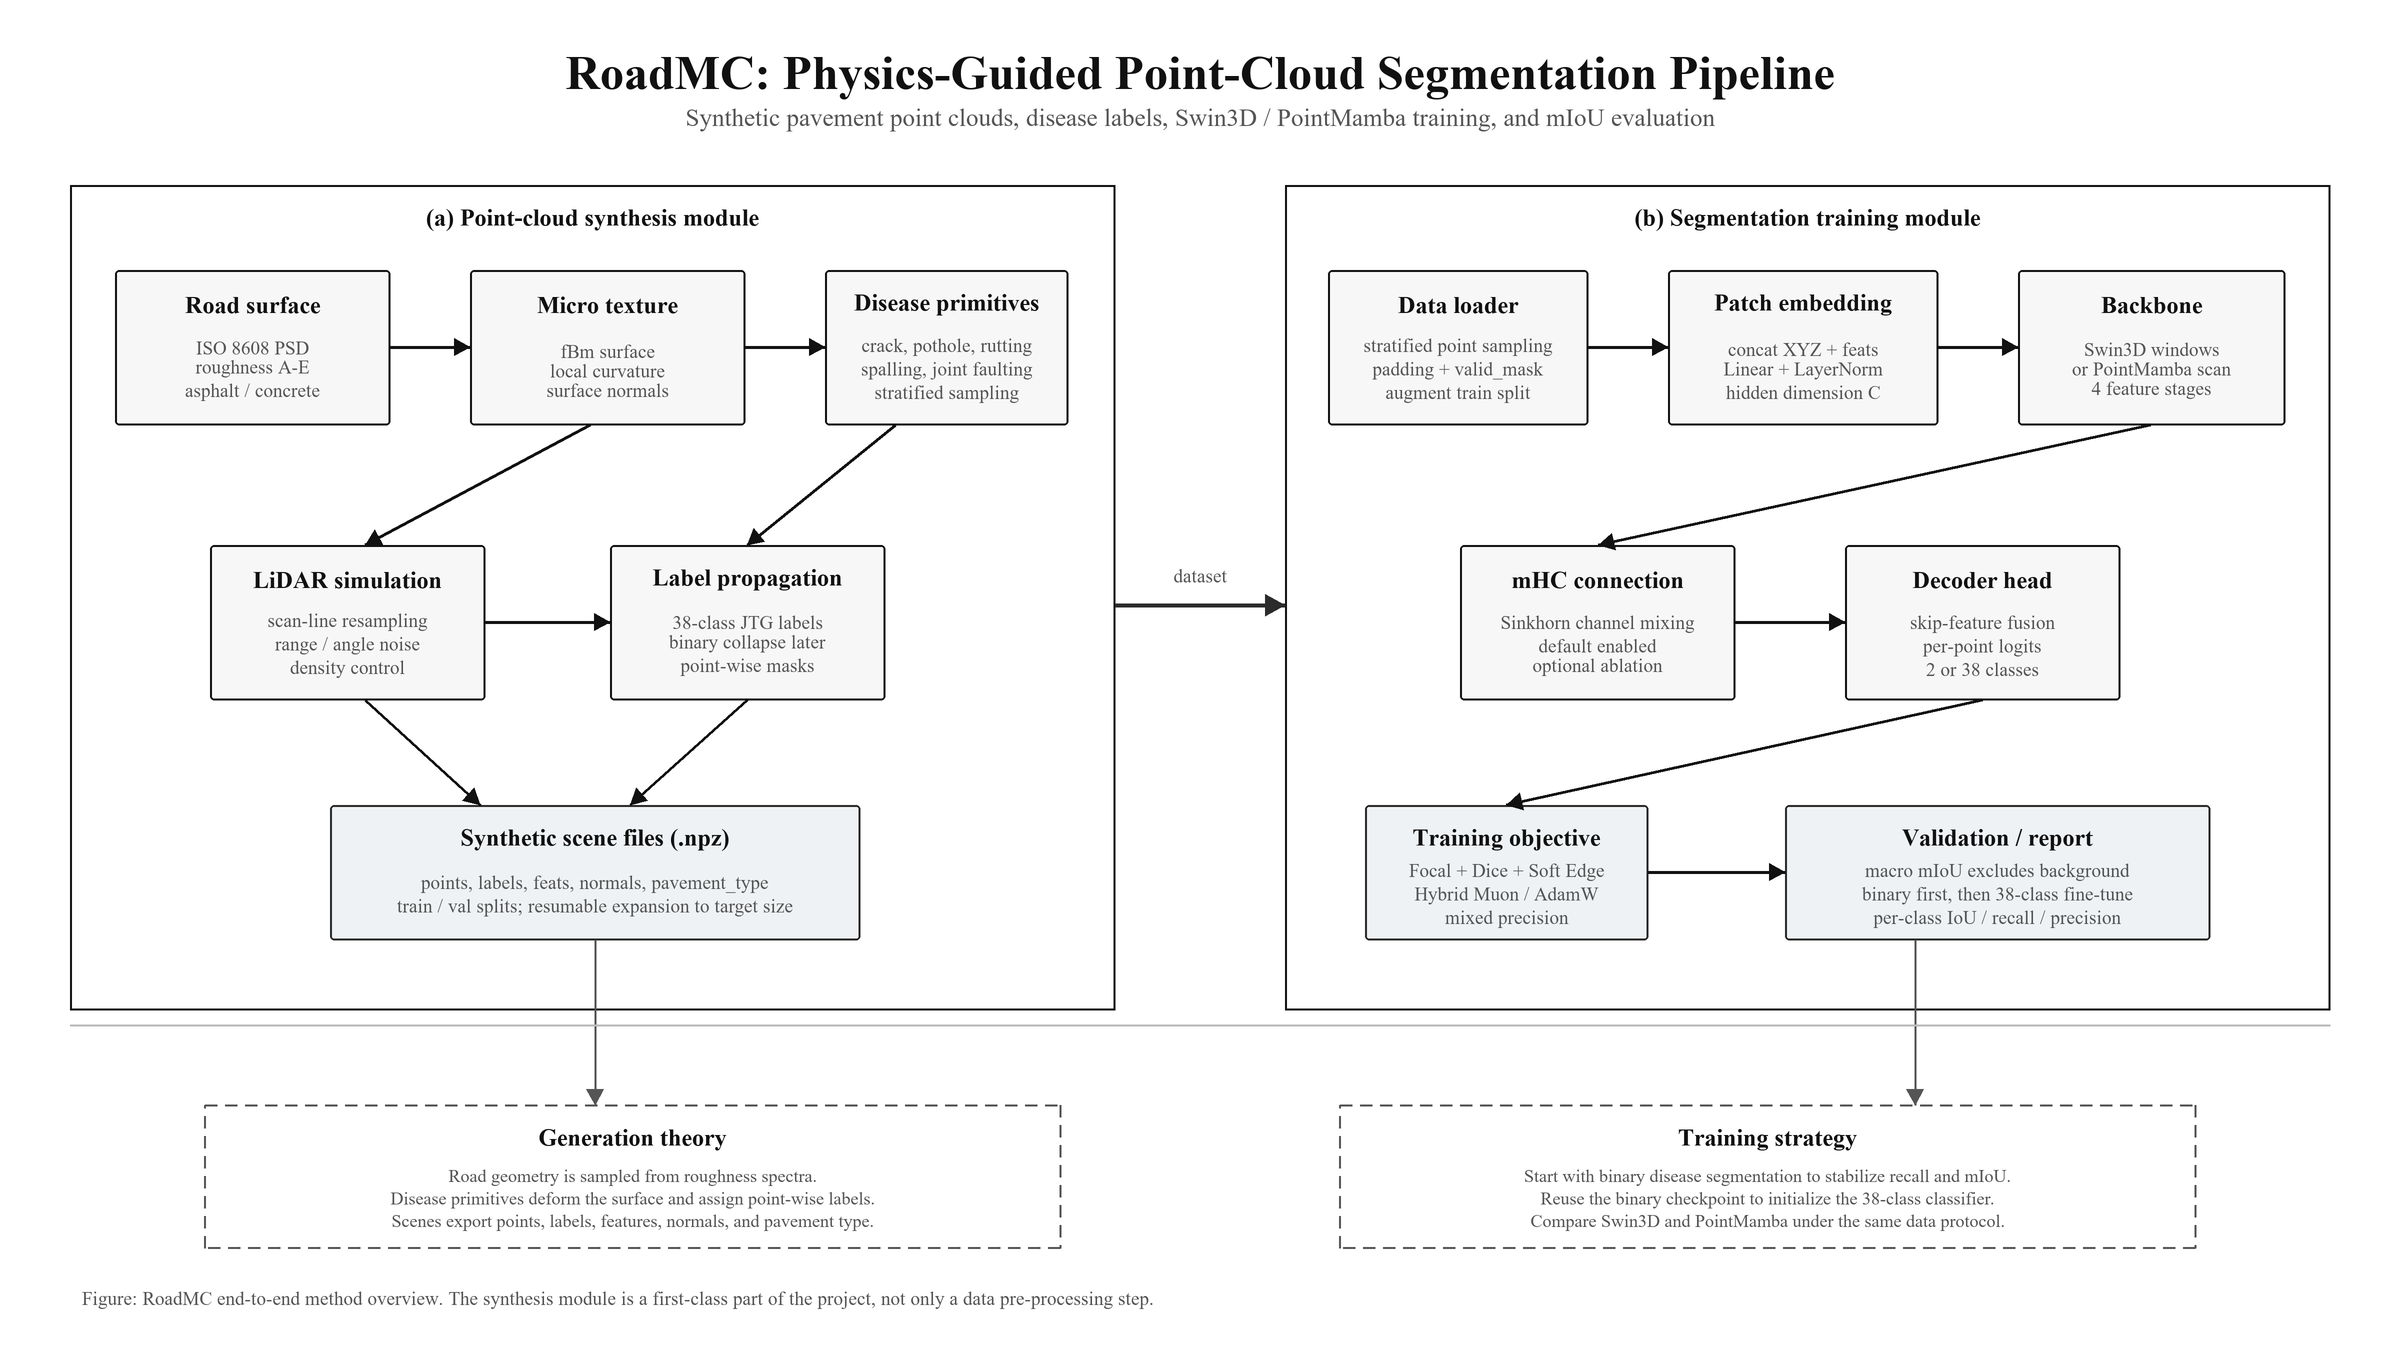
\includegraphics[width=\textwidth]{roadmc_method.png}
  \caption{RoadMC end-to-end overview. The synthesis module is a first-class part of the method, not merely a preprocessing step.}
  \label{fig:overview}
\end{figure*}

\section{Experimental Setup}
Unless otherwise noted, the reported binary experiments use 600 synthetic training scenes and 150 validation scenes. Each scene is limited to 512 sampled points for the reported short-run experiments, with batch size 4, learning rate $3 \times 10^{-4}$, mixed precision, and Muon as the default optimizer. The weighted binary setting uses class weights $\{1.0, 2.5\}$ for background and disease, respectively.

Table~\ref{tab:setup} summarizes the main configuration.

\begin{table}[t]
\centering
\caption{Binary training configuration used in the reported experiments.}
\label{tab:setup}
\small
\begin{tabular}{p{0.34\columnwidth}p{0.56\columnwidth}}
\toprule
Dataset & 600 train / 150 val synthetic scenes \\
Input points & 512 max points per scene \\
Batch size & 4 \\
Optimizer & Muon with AdamW fallback \\
Backbone & Swin3D or PointMamba \\
mHC & Enabled by default \\
Binary class weights & $\{1.0, 2.5\}$ \\
\bottomrule
\end{tabular}
\end{table}

\section{Results}
Table~\ref{tab:results} reports the main validation result and a small backbone comparison. The strongest binary checkpoint comes from Swin3D with mHC and calibrated thresholding. On the same held-out synthetic validation split, the best operating point reaches 0.7319 mIoU, with disease IoU 0.7052, precision 0.9039, and recall 0.7624.

\begin{table*}[t]
\centering
\caption{Pilot results on the synthetic validation set and quick-run backbone comparison.}
\label{tab:results}
\small
\setlength{\tabcolsep}{4pt}
\resizebox{\textwidth}{!}{%
\begin{tabular}{l l l l l}
\toprule
Setting & Protocol & Metric(s) & Value(s) & Notes \\
\midrule
Swin3D + mHC & Best calibrated checkpoint & mIoU / disease IoU / precision / recall & 0.7319 / 0.7052 / 0.9039 / 0.7624 & Best threshold near $\tau \approx 0.44$ \\
PointMamba + mHC & 200-step binary run & final val mIoU / avg loss & 0.5671 / 0.8949 & Binary weights 1.0/2.5 \\
Swin3D + mHC & 500-step quick run & avg loss / elapsed & 3.7884 / 115.47 s & Lower loss, slower wall time \\
PointMamba + mHC & 500-step quick run & avg loss / elapsed & 4.0206 / 103.25 s & Faster wall time \\
\bottomrule
\end{tabular}%
}
\end{table*}

The results suggest a clear split between accuracy and efficiency. Swin3D tends to achieve the best calibrated binary validation score, while PointMamba is consistently faster in quick runs. This makes PointMamba a promising candidate for large-scale training or tighter GPU budgets, but the current implementation still benefits from additional tuning before it can surpass Swin3D on accuracy.

The 38-class setting remains an ongoing challenge. In short runs, the classifier often collapses to background or over-predicts a small subset of defect classes, indicating that fine-grained recognition requires either stronger class balancing, longer training, or a staged curriculum that moves through intermediate taxonomies.

\section{Discussion}
The project logs indicate that binary segmentation is already usable as a stable intermediate stage, while 38-class segmentation remains difficult because of severe long-tail imbalance. This is not a failure of the synthesis pipeline; on the contrary, it shows why the generator matters. The better the geometry prior and the better the label balance, the more likely the downstream model can learn thin and sparse defects.

Several next steps follow naturally. First, the synthetic corpus should be expanded to around 5000 scenes. Second, the binary stage should be tightened with threshold calibration and systematic class-weight sweeps. Third, the 38-class problem should be tackled with staged training, where the backbone is first stabilized on binary disease detection before fine-grained defect heads are introduced. Finally, real-road loading and domain adaptation can be added once the synthetic pipeline is mature enough to serve as a reliable pretraining source.

\section{Conclusion}
RoadMC couples physics-guided synthetic point-cloud generation with modular point-cloud segmentation. The current codebase provides a complete path from road surface synthesis to binary defect segmentation and an expandable route toward 38-class fine-grained recognition. On the held-out synthetic validation split, calibrated binary inference already reaches 0.7319 mIoU, confirming that the generated data carries enough structure to train a meaningful defect detector. The remaining challenge is not whether the framework can learn, but how to scale it to rarer classes and real-world distributions without losing stability.

\begin{thebibliography}{99}

\bibitem{pointnetpp}
C.~R. Qi, L. Yi, H. Su, and L.~J. Guibas, ``PointNet++: Deep hierarchical feature learning on point sets in a metric space,'' \emph{Advances in Neural Information Processing Systems}, vol.~30, 2017.

\bibitem{swin3d}
Y.-Q. Yang, Y.-X. Guo, and Y. Liu, ``Swin3D: A pretrained transformer backbone for 3D indoor scene understanding,'' \emph{arXiv preprint arXiv:2304.06906}, 2023.

\bibitem{pointmamba}
D. Liang \emph{et al.}, ``PointMamba: A simple state space model for point cloud analysis,'' \emph{arXiv preprint arXiv:2402.10739}, 2024.

\bibitem{mhc}
Z. Xie \emph{et al.}, ``mHC: Manifold-constrained hyper-connections,'' \emph{arXiv preprint arXiv:2512.24880}, 2025.

\bibitem{focal}
T.-Y. Lin \emph{et al.}, ``Focal loss for dense object detection,'' in \emph{Proc. IEEE Int. Conf. Computer Vision (ICCV)}, 2017, pp.~2980--2988.

\end{thebibliography}

\end{document}
